\section{Results}\label{sec:results}
%Mention something about the distribution of the data? And choice of baseline model.
% ==================================================================
%
% Jo writes here
% Decision tree 
% - performance
\subsection{Decision tree and AdaBoost (classical features)}
We started by performing a grid search for the decision tree, using the metadata from the PlanktoScope images. The parameters tested and optimal parameters can be found in Table \ref{tab:params_tree}. Since max depth was set, the models were trained using a pre-pruning method. To evaluate the model performance we used a 10-fold cross-validation and the accuracy score as evaluation metric.
\begin{table}[h]
    \centering
    \begin{tabular}{ccc}
        \hline
        \verb|max_depth| \, & \verb|min_samples_split| \, & \verb|criterion| \\
        \hline 
        $5$ & $5$ & \verb|gini|$^*$ \\
        $10^*$ & $10$ & \verb|entropy| \\
        $15$ & $15$ & \\
        $20$ & $20^*$ & \\
        \hline
    \end{tabular}
    \caption{Parameters tested when performing a grid search for the decision tree method, where * marks the best results. The models were trained and tested on the metadata from the PlanktoScope}
    \label{tab:params_tree}
\end{table}

The optimal parameters show that the best criterion for splitting is gini, with a max depth of $10$ and a minimum of $20$ samples per split. The accuracy on both train and test data was approx. $78\%$, indicating a well fit model with a balance between complexity and fit. 
We continued with a model using the optimal parameters, and plotted a confusion matrix to investigate the predicted labels. The result is shown in Figure
% Performance using optimal parameters
\begin{figure}
    \centering
    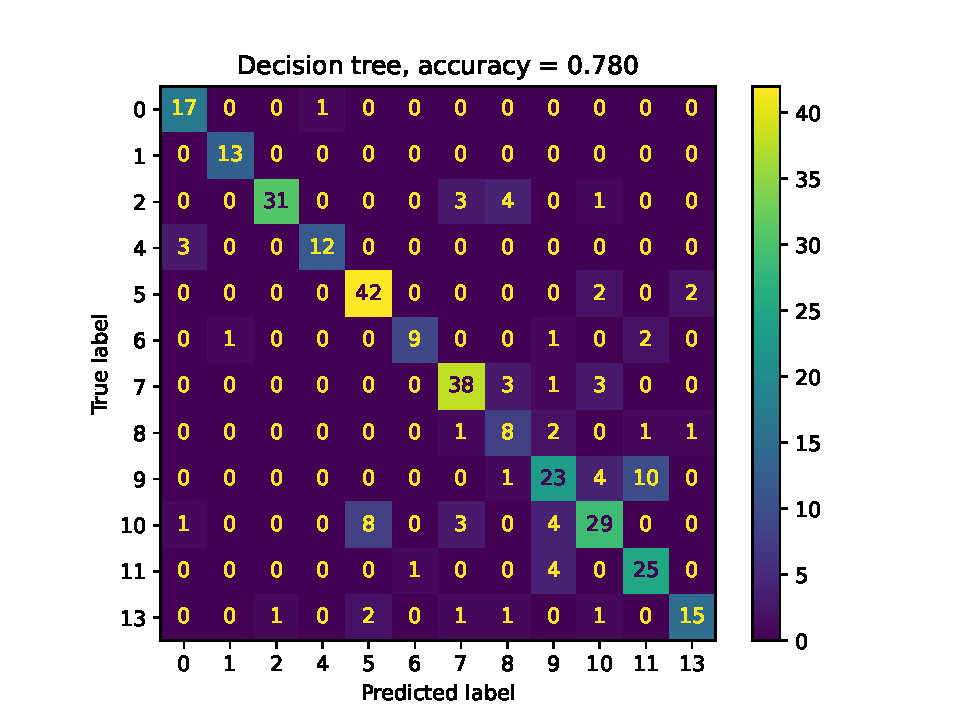
\includegraphics[width=\linewidth]{latex/figures/cm_tree_planktoscope_metadata.pdf}
    \caption{Caption}
    \label{fig:cm_tree_metadata}
\end{figure}

% Adaboost 
% - grid search results
% - performance
To explore the potential of performance increase, we continued with the AdaBoost method using decision tree as the weak classifier. As for the decision tree, we performed a grid search using the parameters found in Table \ref{tab:params_adaboost}. We used the same data as in previous grid search, continued with entropy as criterion for splitting, and the same model evaluation method.
\begin{table}[h]
    \centering
    \begin{tabular}{ccc}
        \hline
        \verb|max_depth| \, & \verb|n_estimators| \, & \verb|learning_rate| \\
        \hline 
        $1$ & $100$ & $0.001$ \\
        $2^*$ & $500$ & $0.01$ \\
         & $1000^*$ & $0.1$ \\
         & & $1.0^*$ \\
        \hline
    \end{tabular}
    \caption{Parameters tested when performing a grid search for the AdaBoost method, where * marks the best results. The models were trained and tested on the metadata from the PlanktoScope}
    \label{tab:params_adaboost}
\end{table}
% Waiting for results XP

%Results for dino features after dino results :)
% ==================================================================

% ==================================================================
%
% EB writes here
%
\subsection{DINOv2 ViT}
We extracted 384 features for each of the 2061 images [camera type here], inserted them into a design matrix with rows containing a numerical feature and columns containing the image they originated from. The resulting 2961 x 384 matrix was then standardized and reduced with either PCA with 70 principal components, or UMAP with 2 embeddings. 

We present the first two components of the PCA plotted against each other in Figure \ref{fig:pca0pca1}, and the embeddings from UMAP in Figure \ref{fig:umap}. Both figures have labeled species data points, but this labels have not been provided for the DINO ViT model and are provided afterwards to see whether the feature representations we've retrieved can be considered good representations.

After analyzing the cumulative variance for each component (Appendix, Figure \ref{fig:cumsumpca}), we saw that including 70 components accounted for just above 85\% of the variance in the design matrix, and the first two components only account for around 26\%. This means that we cannot assume the PC representations to relay significant relationships in our data. 

In Figure \ref{fig:umap} we see clear clusters. We already know that the input images belonged to 14 categories, and yet we count 11 distinct cluster which is also confirmed by the silhouette score for each of the 2-20 KMeans clusters we tested (Appendix, Figure \ref{fig:kmean_sil}). We suspect that the species that have similar feature embeddings might also have some morphological similarities, which is confirmed by looking into some example photos in Figure \ref{fig:pseudo+empty}. 

\begin{figure}[H]
    \centering
    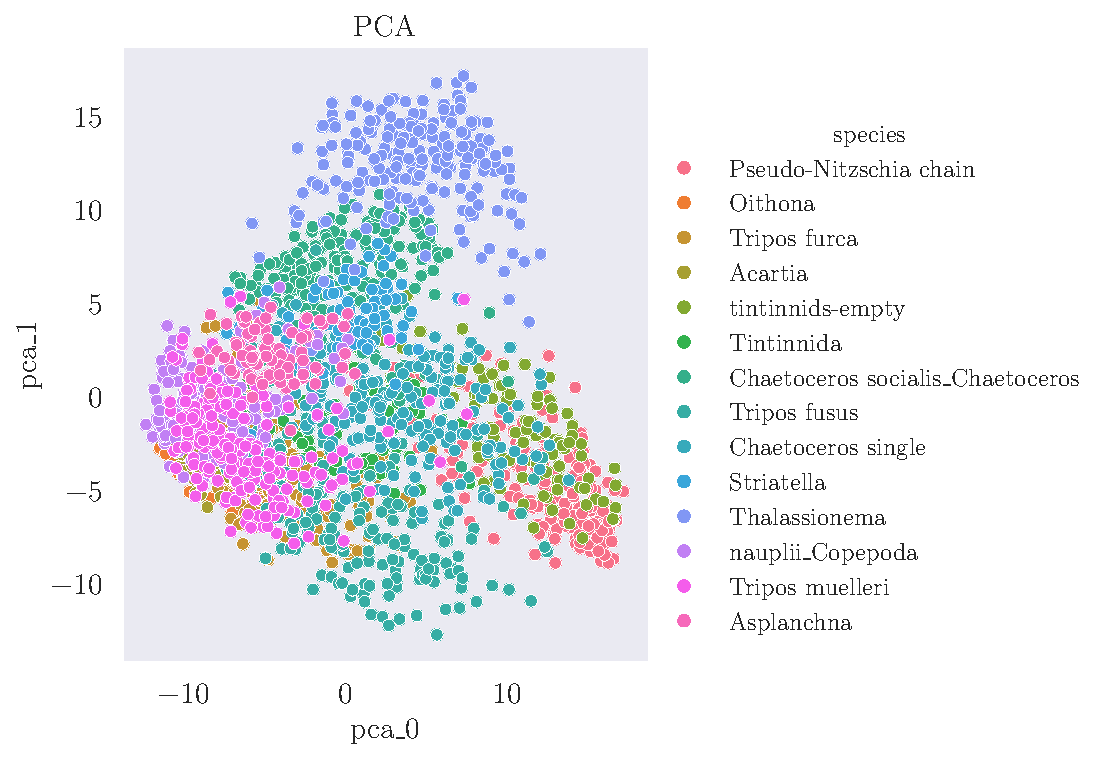
\includegraphics[width=1.1\linewidth]{examples/tests_eb/figs/pca0_pca1.pdf}
    \caption{The two first principal components out of 70 plotted against each other. Already here we can see some weak signs of clusters}
    \label{fig:pca0pca1}
\end{figure}

\begin{figure}[H]
    \centering
    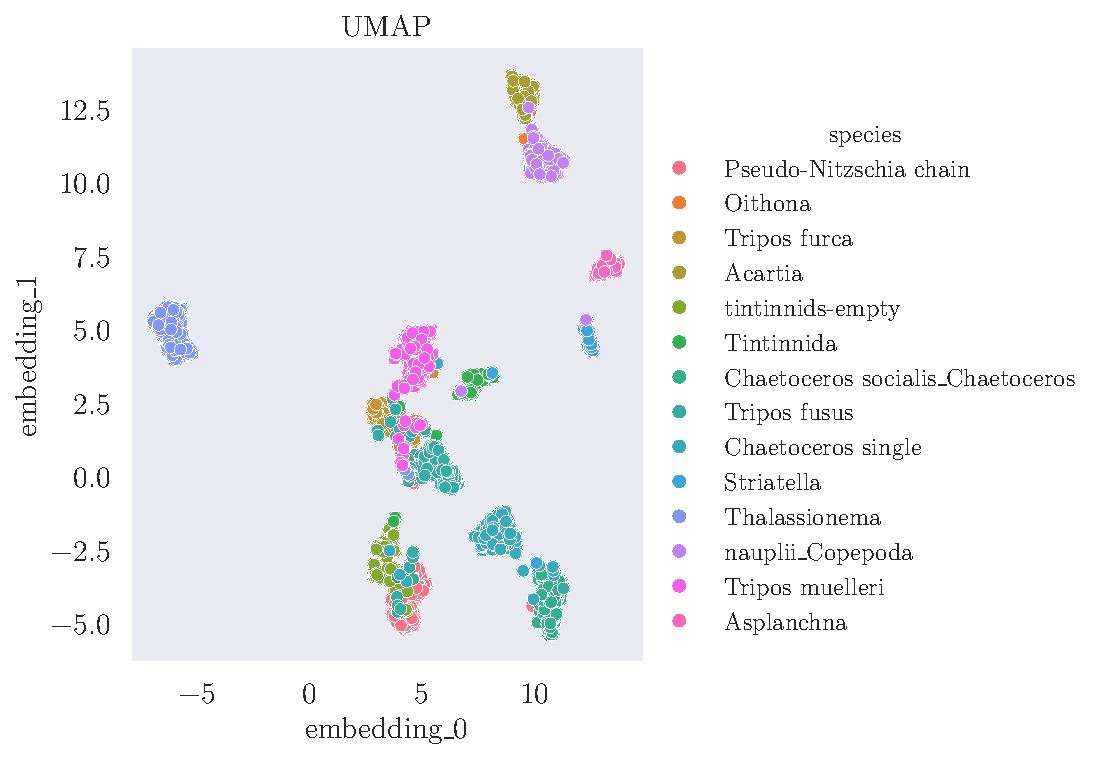
\includegraphics[width=1.1\linewidth]{examples/tests_eb/figs/umap.pdf}
    \caption{A UMAP plot to explore non-linear relations in our data (TODO - read up on UMAP). Here we can clearly see how our extracted features cluster together, yet we still do not have 14 distinct clusters.}
    \label{fig:umap}
\end{figure}

\begin{figure}[H]
    \centering
    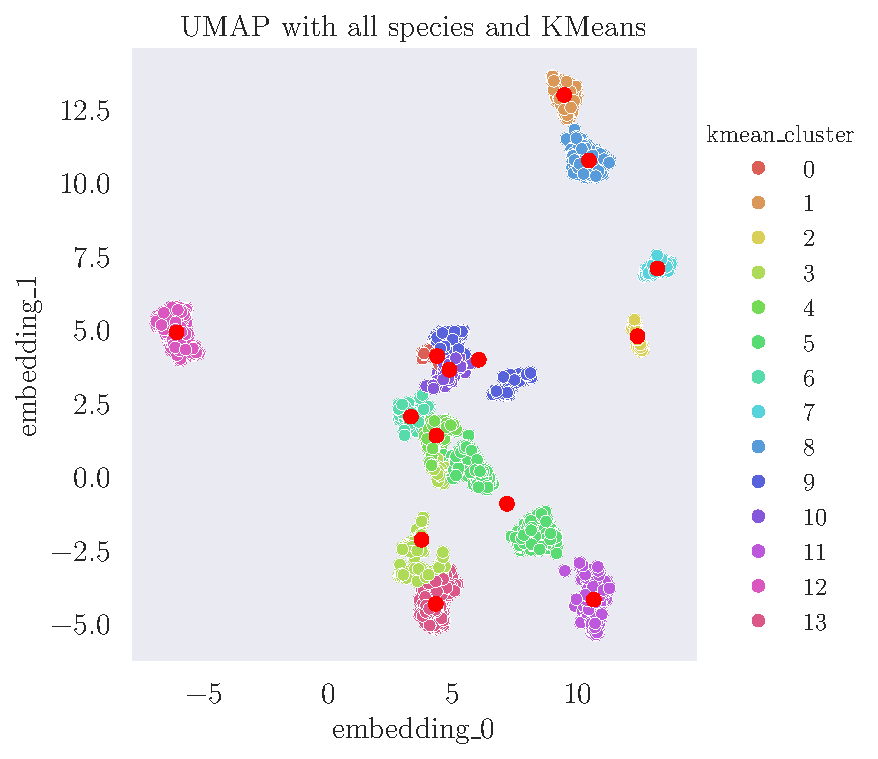
\includegraphics[width=1\linewidth]{latex/figures/kmeans_cluster_umap_on_all_species.pdf}
    \caption{A UMAP with KMeans centroids, which were set to 14 clusters although silhouette coefficients suggested 11. We can clearly see how some centroids are quite close, and arguably even too close for any distinction of the two clusters. We can also see how there appears to be some non-logical centroid placements, as is the case with centroids around 5 (green) and 9 (blue).}
    \label{fig:14-mer-umap}
\end{figure}

\begin{figure}[H]
    \centering
    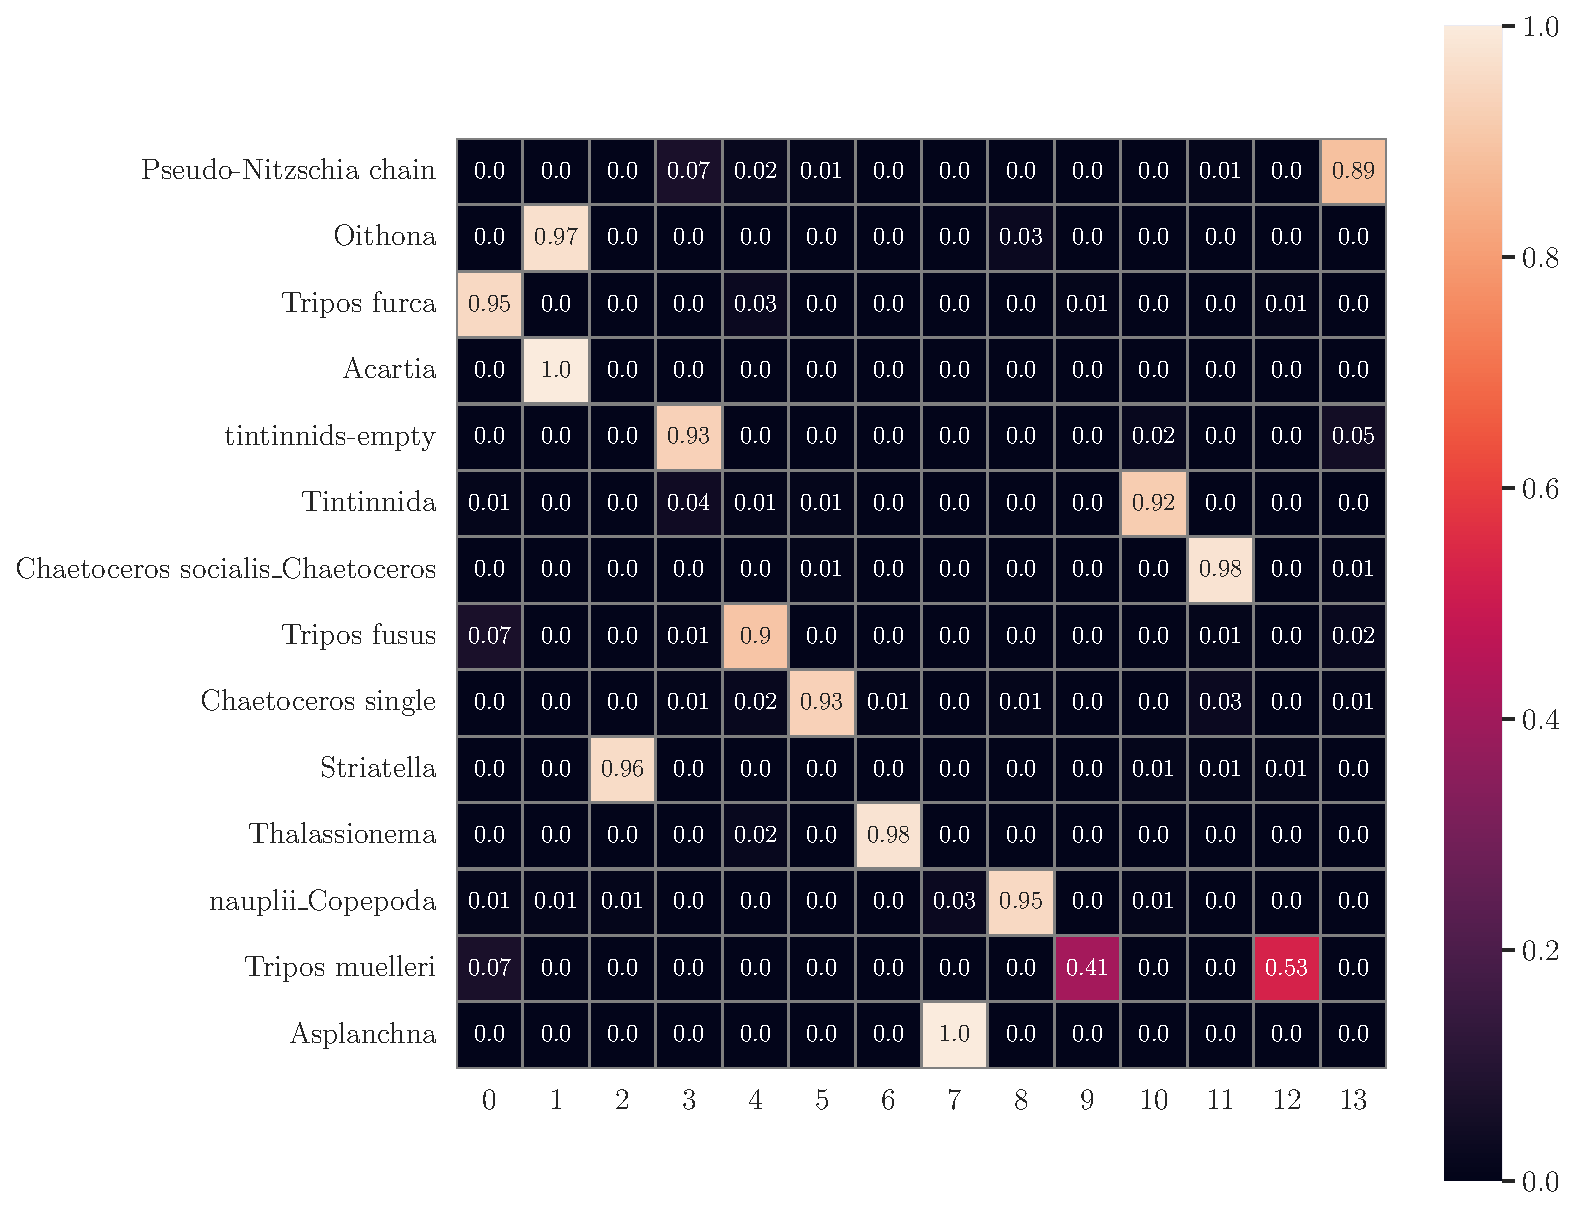
\includegraphics[width=1\linewidth]{latex/figures/dinov2_confmat.pdf}
    \caption{A pseudo-confusion matrix of the unlabeled k-mer centrods and the percentage of species classified withing a k-mer. The total sum of each row adds up to one, so each row presents the distribution of a species within the 14 k-mer clusters. We can see here how \textit{Tripos muelleri} are placed in the dubious 9-mer cluster mentioned in Figure \ref{fig:14-mer-umap}}
    \label{fig:dinov2-confusion}
\end{figure}

\begin{figure}[H]
    \centering
    % Første subfigur
    \begin{subfigure}[b]{0.32\linewidth}
        \centering
        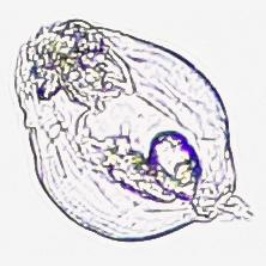
\includegraphics[width=\linewidth]{examples/tests_eb/figs/plankton_examplebatch/asplanktia.png}
        \caption{Species Asplanchna}
        \label{fig:asplanch}
    \end{subfigure}
    % Andre subfigur
    \begin{subfigure}[b]{0.32\linewidth}
        \centering
        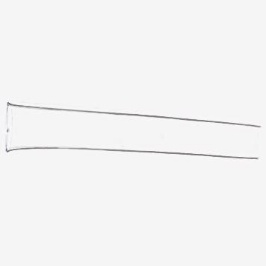
\includegraphics[width=\linewidth]{examples/tests_eb/figs/plankton_examplebatch/empty.jpg}
        \caption{Species Tintinnids-empty}
        \label{fig:empty}
    \end{subfigure}
    % Tredje subfigur
    \begin{subfigure}[b]{0.32\linewidth}
        \centering
        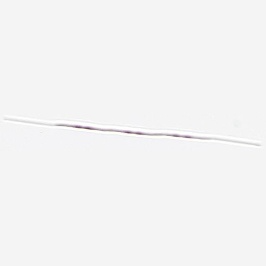
\includegraphics[width=\linewidth]{examples/tests_eb/figs/plankton_examplebatch/pseudo.png}
        \caption{Species Pseudo-Nitzschia}
        \label{fig:pseudo}
    \end{subfigure}
    \caption{In (a), we see an example of a species that has a clear, separate cluster in Figure \ref{fig:umap}. We compare this to (b) and (c), which seemingly cluster together in the same figure.}
    \label{fig:grid}
\end{figure}

Just for fun, we looked into the species that would have been misclusteded if we used KMeans clustering on the two similar species mentioned in Figure \ref{fig:grid}. 

\begin{figure}[H]
    \centering
    \begin{subfigure}[b]{1\linewidth}
        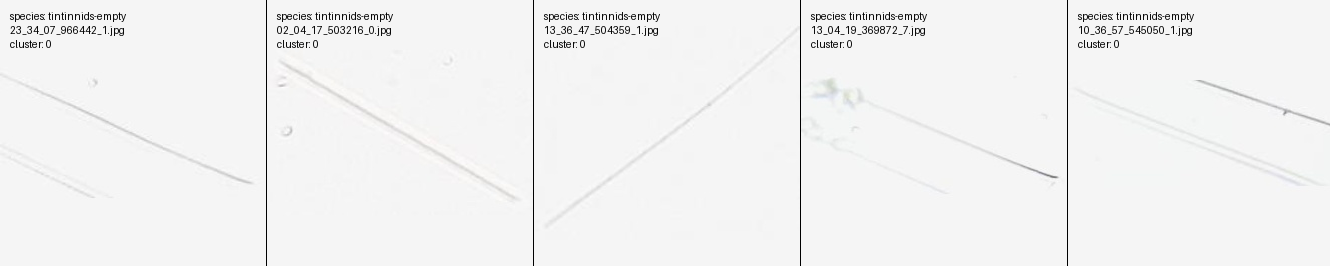
\includegraphics[width=\linewidth]{examples/tests_eb/figs/misclustered_empty.png}
        \caption{Tintinnids-empty that have clustered with Pseudo-Nitzchia chains according to simple K-means clustering of an isolated selection of UMAP embeddings for the two species.}
    \end{subfigure}
    
    \vspace{1em}
    
    \begin{subfigure}[b]{1\linewidth}
        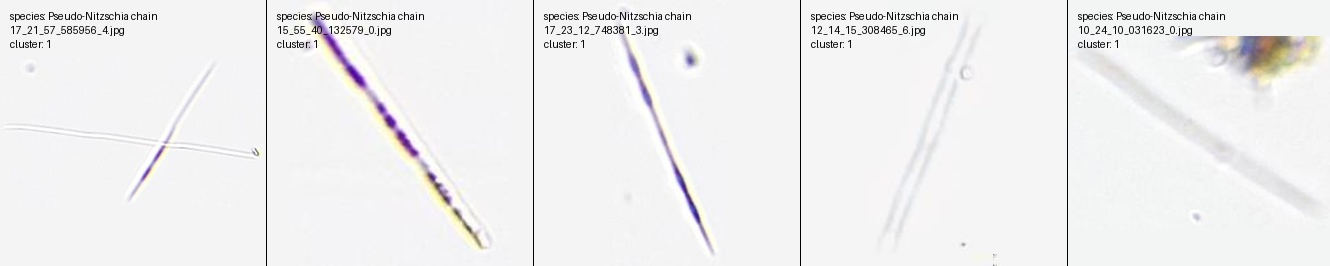
\includegraphics[width=\linewidth]{examples/tests_eb/figs/misclustered_pseudo-nitz.png}
        \caption{Pseudo-Nitzschia chains that have clustered with Tintinnids-empty according to simple K-means clustering of an isolated selection of UMAP embeddings for the two species.}
    \end{subfigure}
    \caption{We compare some of the species that seem to cluster together in Figure \ref{fig:umap} to explore whether the original labels are incorrect or if our DINOv2 fails to discern between the two species. The clustering process demonstrated in Figure \ref{fig:misclustering_process} in our Appendix.}
    \label{fig:misclusters}
\end{figure}


% ==================================================================